\documentclass[zihao=-4,a4,seagreen,openany]{ibook}
\usepackage{bookmark}
\usepackage{tikz}
\usepackage{xcolor} 
\usepackage{listings}
\usepackage{paralist}
\usetikzlibrary{patterns}
\usepackage{pgfplots}
\usetikzlibrary{arrows,shapes,chains}
\usetikzlibrary{calc}
\newcommand{\fira}{\fontspec{Cousine for Powerline}}
\renewcommand{\lstlistlistingname}{代码索引}
\AtBeginEnvironment{lstlisting}{\linespread{1.05}}

\definecolor{CPPLight}  {HTML} {686868}
\definecolor{CPPSteel}  {HTML} {888888}
\definecolor{CPPDark}   {HTML} {262626}
\definecolor{CPPBlue}   {HTML} {4172A3}
\definecolor{CPPGreen}  {HTML} {487818}
\definecolor{CPPBrown}  {HTML} {A07040}
\definecolor{CPPRed}    {HTML} {AD4D3A}
\definecolor{CPPViolet} {HTML} {7040A0}
\definecolor{CPPGray}  {HTML} {B8B8B8}
\lstdefinestyle {code} {
    language=c++,                                        % 设置语言
    columns=fixed,       
    numbers=left,                                        % 在左侧显示行号
    frame=none,                                          % 不显示背景边框
    basicstyle = \fira,
    backgroundcolor=\color[RGB]{245,245,244},            % 设定背景颜色
    keywordstyle=\color[RGB]{40,40,255}\bfseries,        % 设定关键字颜色
    ndkeywordstyle=\color{CPPViolet},
    % otherkeywordstyle=\color{CPPGreen}
    identifierstyle=\color{CPPBrown},
    numberstyle=\footnotesize\color{black!50},           % 设定行号格式
    commentstyle=\it\color[RGB]{0,96,96},                % 设置代码注释的格式
    stringstyle=\rmfamily\color{CPPGreen},            % 设置字符串格式
    showstringspaces=false,                              % 不显示字符串中的空格
    morekeywords={alignas,continute,friend,register,true,alignof,decltype,
    reinterpret_cast,try,asm,defult,if,return,typedef,auto,delete,inline,short,
    typeid,bool,int,signed,typename,break,double,long,sizeof,union,case,
    dynamic_cast,mutable,static,unsigned,catch,else,namespace,static_assert,using,
    char,enum,new,static_cast,virtual,char16_t,char32_t,explict,noexcept,struct,
    void,export,nullptr,switch,volatile,class,extern,operator,template,wchar_t,
    const,false,private,this,while,constexpr,float,protected,thread_local,
    const_cast,for,public,throw,std},
}

\lstset{style=code}

\begin{document}

\frontmatter
\tableofcontents

\mainmatter
\part{设计}

\chapter{背景分析}

在现代计算机中,求交并集是不可缺少的操作,能快速处理交集和并集运算是计算机底层的算法的要求。%

对于已排序的序列进行求交运算是一个简单的问题,并且有$O(n)$的时间复杂度上限。


\chapter{功能设计}

\section{题意转化}
题目给定已知两个非降序链表序列$S_1$和$S_2$,设计函数构造出$S_1$和$S_2$的交集新链表$S_3$。%
因为{\kaishu 链表}、{\kaishu 非降序}两个条件已经限定,因此求交集更多是一个{\kaishu 算法},而非数据结构%
的问题。项目中的链表在数据存储中可能为以下形式,本题只需要一个单向连接的链表就能完成。

\newcommand{\data[1]}{
      #1 \nodepart{second}
      \phantom{\texttt{NULL}}
    }

\begin{figure}[H]
    \tikzstyle{ptr}  = [draw, -{Stealth[scale=1.0]}, blue]
    \tikzstyle{head} = [rectangle, draw, text height=3mm, text width=3mm,
                        text centered, node distance=3cm, inner sep=0pt]
    \tikzstyle{data} = [rectangle split, rectangle split parts=2, draw, node distance=2.5cm, 
                        text centered, minimum height=3em]
    \centering
    \begin{tikzpicture} [node distance=2cm, auto]
        \node[head, label=below:phead] (head) {};
        \node[data, right of=head] (A) {\data[0]};
        \node[data, right of=A] (B) {\data[1]};
        \node[data, right of=B] (C) {\data[5]};
        \node[data, right of=C] (D) {\data[6]};
        \node[data, right of=D] (E) {-1 \nodepart{second} \texttt{nullptr}};
        
    
        \draw[fill] (head.center) circle (0.05);
    
        \path[ptr] (head.center) --++(right:7.5mm) |- (A.text west);
        \draw[fill] ($(A.south)!0.5!(A.text split)$) circle (0.05);
        \draw[ptr] ($(A.south)!0.5!(A.text split)$) --++(right:10mm) |- (B.text west);
        \draw[fill] ($(B.south)!0.5!(B.text split)$) circle (0.05);
        \draw[ptr] ($(B.south)!0.5!(B.text split)$) --++(right:10mm) |- (C.text west);
        \draw[fill] ($(C.south)!0.5!(C.text split)$) circle (0.05);
        \draw[ptr] ($(C.south)!0.5!(C.text split)$) --++(right:10mm) |- (D.text west);
        \draw[fill] ($(D.south)!0.5!(D.text split)$) circle (0.05);
        \draw[ptr] ($(D.south)!0.5!(D.text split)$) --++(right:10mm) |- (E.text west);
    
    \end{tikzpicture}
    \caption{单链表结构示意图}
\end{figure}

解决的关键在以何种方式遍历这两个链表才能达到较好的时间复杂度。

如果对 $S_1$ 中每一个元素,都去检查 $S_2$ 中是否含有该元素,设 $n = S_1.size()$ ,%
$m = S_1.size()$,则该算法是一个时间复杂度 $O(n \times m)$ 的算法,而且没有用上 {\kaishu 非降序} 这个条件。

如果简单地用上{\kaishu 非降序}条件:在检查 $S_2$ 中是否含有 $S_1$ 中某元素$x$时,因为 $S_2$ 已经有序,因此当比较到%
$S_2$ 中元素大于 $x$ 时,就可以停止比较并且这表示 $x$ 并不在 $S_2$ 中。这种算法还是有退化成 $n \times m$ 次比较的可能%
(在 $S_1$ 中元素都大于等于 $S_2$ 中元素时),并且平均时间复杂度也还是 $O(n \times m)$。复杂度没有下降的原因在于 $S_1$ %
的非降序条件依然没有用上。

用上所有条件,该算法的时间复杂度为 $O(n + m)$ 。具体的做法是:两个指针 \lstinline{p}、\lstinline{q} 开始时指向$S_1$和$S_2$%
的头节点,接下来做以下循环:\label{logic}
\begin{itemize}
    \item 如果 \lstinline{p} 或 如果 \lstinline{q} 为空,停止循环。
    \item 如果 \lstinline{p}、\lstinline{q} 节点的值相等,将该值置入 $S_3$,\lstinline{p}、\lstinline{q}指下一个节点;
    \item 如果 \lstinline{p} 节点的值大于 \lstinline{q} 的值,\lstinline{p} 指下一个节点。
    \item 如果 \lstinline{q} 节点的值大于 \lstinline{p} 的值,\lstinline{q} 指下一个节点。
\end{itemize}

本题考虑了一种极端情况:当输入的数据大于所有 \emph{C++} 可以表示的整数数据类型时,一个输入只能被拆做两个或多个来读取。所以我引入了%
\emph{Java} 中 \lstinline{BigInteger} 的设计,实现了一个不管多大整数序列都能存储的数据类型。该数据类型重载了输入输出、大小比较%
以及检查数据是否合理。链表中存放的就是该数据结构,会在\textbf{实现}部分详细说明。

下一节将具体介绍这样的逻辑和解题过程中数据内部结构。

\section{逻辑功能}

\section{流程图}

\tikzstyle{startstop} = [rectangle, rounded corners, minimum width = 2cm, 
        minimum height=1cm, text centered, draw = black, fill = red!40,
        font = {\bfseries}]
    \tikzstyle{io} = [trapezium, trapezium left angle=70, trapezium right angle=110, 
    minimum width=2cm, minimum height=1cm, text centered, draw=black, fill = blue!40]
    \tikzstyle{process} = [rectangle, minimum width=3cm, minimum height=1cm, text centered, draw=black, fill = yellow!50]
    \tikzstyle{condition} = [diamond, aspect = 3, text centered, draw=black, fill = green!30]
    \tikzstyle{arr} = [->, >=stealth, thick]

\subsection{输入逻辑}
因为本题使用了大整数,且题目也限定了一些重要的先决条件,所以在正式处理序列求交集时需要对序列做输入检查,检查流程如下。
{
    \begin{figure}[H]
        \centering
        \begin{tikzpicture}
            \node [startstop] (start) {开始};
            \node [io, below=0.6cm of start] (input) {输入序列};
            \node [condition, below=0.6cm of input] (cond1) {序列中每个数都是正整数或$-1$};
            \node [condition, below=0.6cm of cond1] (cond2) {序列非降序};
            \node [startstop, below=0.6cm of cond2] (end) {返回有效序列};
            \node [process, left=1.0cm of cond1] (aban) {抛弃序列};

            \draw [arr] (start) -- (input);
            \draw [arr] (input) -- (cond1);
            \draw [arr] (cond1) -- node[anchor=west] {是} (cond2);
            \draw [arr] (cond2) -- node[anchor=west] {是} (end);
            \draw [arr] (cond1) -- node[anchor=south] {否} (aban);
            \draw [arr] (cond2) -| node[anchor=north] {否} (aban);

            \draw [arr] (aban) |- node {} ($ (input.north) + (0, 0.3) $);

        \end{tikzpicture}
        \caption{输入序列数据逻辑}
    \end{figure}
}

\subsection{总体逻辑}
本部分与第\ref{logic}小节叙述的过程相同,用两个指针来按顺序单次遍历两个序列,从而只要访问 $n+m$ 次序列中的元素%
就能得到结果 $S_3$。开始时我们将 $S_3$ 设置成空指针,把值置入$S_3$新节点时先给节点分配空间,再用值初始化该节点。

用流程图表示如下:\\

\begin{figure}[H]
    \centering
    \begin{tikzpicture}
        \node [startstop] (start) {开始};
        \node [io, below=0.6cm of start] (input) {输入序列$S_1$、$S_2$};
        \node [process, below=0.6 of input] (set) {\lstinline{p}、\lstinline{q}指向$S_1$、$S_2$头节点};
        \node [condition, below=0.6cm of set] (condEnd) {\lstinline{p}或\lstinline{q}不为空};
        \node [startstop, right=1.2cm of condEnd] (end) {返回$S_3$};
        \node [condition, below=0.6cm of condEnd] (condEq) {\lstinline{p}、\lstinline{q}值相等};
        \node [process, left=1.0cm of condEq] (in) {将\lstinline{p}值置入$S_3$};
        \node [process, above=.3cm of in] (adPQ) {\lstinline{p = p.next;q = q.next}};
        \node [condition, below=0.6cm of condEq] (condLt) {\lstinline{p}值比\lstinline{q}小};
        \node [process, below=.6cm of condLt, xshift = -2.5cm] (adP) {\lstinline{p = p.next}};
        \node [process, below=.6cm of condLt, xshift = 2.5cm] (adQ) {\lstinline{q = q.next}};
        \node [below=2cm of condLt, transparent] (anchor) {};

        \draw [arr] (start) -- (input);
        \draw [arr] (input) -- (set) -- (condEnd) -- (condEq) -- (condLt);
        \draw [arr] (set) -- (condEnd);
        \draw [arr] (condEnd) -- node[anchor=west] {是} (condEq);
        \draw [arr] (condEnd) -- node[anchor=south] {否} (end);
        \draw [arr] (condEq) -- node[anchor=south] {是} (in);
        \draw [arr] (in) -- (adPQ);
        \draw [arr] (adPQ) |- ($(condEnd.north) + (0, .3)$);
        \draw [arr] (condEq) -- node[anchor=west] {否} (condLt);
        \draw [arr] (condLt) -| node[anchor=east] {是} (adP);
        \draw [arr] (condLt) -| node[anchor=west] {否} (adQ);
        \draw [thick] (adQ) |- (anchor.west);
        \draw [thick] (adP) |- (anchor.west);
        \draw [thick] (anchor.east) --  ($ (anchor.east) + (-8, 0) $) node {} ;
        \draw [arr] ($ (anchor.east) + (-8, 0) $) |- ($(condEnd.north) + (0, 0.3)$);
    \end{tikzpicture}
    \caption{总体逻辑}
\end{figure}


\section{数据内部结构示意}

以下是某时刻两序列链表$S_1$、$S_2$和结果链表$S_3$中的可能状态。

\begin{figure}[H]
    \tikzstyle{ptr}  = [draw, -{Stealth[scale=1.0]}, blue]
    \tikzstyle{head} = [rectangle, draw, text height=3mm, text width=3mm,
                        text centered, node distance=3cm, inner sep=0pt]
    \tikzstyle{data} = [rectangle split, rectangle split parts=2, draw, node distance=2.5cm, 
                        text centered, minimum height=3em]
    \centering
    \begin{tikzpicture} [node distance=2cm, auto]
        \node[head, label=below:$S_1$] (S1head) {};
        \node[data, right of=S1head] (A) {\data[0]};
        \node[data, right of=A] (B) {\data[5]};
        \node[data, right of=B] (C) {\data[6]};
        \node[data, right of=C] (D) {\data[10]};
        \node[data, right of=D] (E) {-1 \nodepart{second} \texttt{nullptr}};
        
    
        \draw[fill] (S1head.center) circle (0.05);
    
        \path[ptr] (S1head.center) --++(right:7.5mm) |- (A.text west);
        \draw[fill] ($(A.south)!0.5!(A.text split)$) circle (0.05);
        \draw[ptr] ($(A.south)!0.5!(A.text split)$) --++(right:10mm) |- (B.text west);
        \draw[fill] ($(B.south)!0.5!(B.text split)$) circle (0.05);
        \draw[ptr] ($(B.south)!0.5!(B.text split)$) --++(right:10mm) |- (C.text west);
        \draw[fill] ($(C.south)!0.5!(C.text split)$) circle (0.05);
        \draw[ptr] ($(C.south)!0.5!(C.text split)$) --++(right:10mm) |- (D.text west);
        \draw[fill] ($(D.south)!0.5!(D.text split)$) circle (0.05);
        \draw[ptr] ($(D.south)!0.5!(D.text split)$) --++(right:10mm) |- (E.text west);


        \node[head, label=below:$S_2$, below=1.5cm of S1head] (S2head) {};
        \node[data, right of=S2head] (A2) {\data[0]};
        \node[data, right of=A2] (B2) {\data[2]};
        \node[data, right of=B2] (C2) {\data[5]};
        \node[data, right of=C2] (D2) {\data[6]};
        \node[data, right of=D2] (E2) {-1 \nodepart{second} \texttt{nullptr}};
        
    
        \draw[fill] (S2head.center) circle (0.05);
    
        \path[ptr] (S2head.center) --++(right:7.5mm) |- (A2.text west);
        \draw[fill] ($(A2.south)!0.5!(A2.text split)$) circle (0.05);
        \draw[ptr] ($(A2.south)!0.5!(A2.text split)$) --++(right:10mm) |- (B2.text west);
        \draw[fill] ($(B2.south)!0.5!(B2.text split)$) circle (0.05);
        \draw[ptr] ($(B2.south)!0.5!(B2.text split)$) --++(right:10mm) |- (C2.text west);
        \draw[fill] ($(C2.south)!0.5!(C2.text split)$) circle (0.05);
        \draw[ptr] ($(C2.south)!0.5!(C2.text split)$) --++(right:10mm) |- (D2.text west);
        \draw[fill] ($(D2.south)!0.5!(D2.text split)$) circle (0.05);
        \draw[ptr] ($(D2.south)!0.5!(D2.text split)$) --++(right:10mm) |- (E2.text west);


        \node[head, label=below:$S_3$, below=1.5cm of S2head] (S3head) {};
        \node[data, right of=S3head] (A3) {\data[0]};
        \node[data, right of=A3] (B3) {5 \nodepart{second} \texttt{nullptr}};
    
        \draw[fill] (S3head.center) circle (0.05);
    
        \path[ptr] (S3head.center) --++(right:7.5mm) |- (A3.text west);
        \draw[fill] ($(A3.south)!0.5!(A3.text split)$) circle (0.05);
        \draw[ptr] ($(A3.south)!0.5!(A3.text split)$) --++(right:10mm) |- (B3.text west);

    
        \node [above=0.6cm of C] (p) {p};
        \node [below=.6cm of D2] (q) {q};
        \draw [ptr] (p) -- (C);
        \draw [ptr] (q) -- (D2);
    \end{tikzpicture}
    \caption{算法数据组织示意图}
\end{figure}

\part{实现}

\chapter{类结构}
由于使用了哈希表,本项目的代码结构较为复杂,因此加以解释。\lstinline{HashTable} 类是仿照 \emph{C++ STL} 源码实现的,其中使用了%
\lstinline{Vector} 类,所以代码中出现在上面的类型(本应该被 \lstinline{#include} 进来)是下面类型的依赖,而不是更重要的意思。%
下面按照一定的逻辑顺序介绍这几个类:

\begin{itemize}
    \item \lstinline{MultiTree} 类\\
    由二叉树存储的多叉树类,遵循“左长子右兄弟”的规则进行存放。每个节点含有三个指针域,分别指向长子、兄弟和父母。
    \item \lstinline{HashTable} 类\\
    其中维护了一个 \lstinline{HashNode} 的 \lstinline{Vector},通过其哈希函数(\lstinline{hash function})完成对\lstinline{Vector}%
    数组的索引。主要通过\lstinline{find} 和 \lstinline{hasKey}索引和判断键的存在与否,通过 \lstinline{insert} 方法插入一个键唯一的对象。%
    通过 \lstinline{erase} 方法抹去一个值。
    \item \lstinline{StringHashMap} 类\\
    包装和特化之后的一个哈希键值对集合,通过字符串进行索引得到对应值,范型参数为值的类型。可以通过\lstinline{find} 和 %
    \lstinline{hasKey}索引和判断键的存在与否,通过 \lstinline{insert} 方法插入一个键唯一的对象。%
    通过 \lstinline{erase} 方法抹去一个值。并且重载了下标运算符 \lstinline{[]},将字符串作为下标可以索引对应的值。
    \item \lstinline{Vector} 类\\
    \lstinline{HashTable} 类用与存放\lstinline{HashNode}的数组,相同哈希值的对象会以链表的方式存放在这个数组的单元里。%
    在\lstinline{HashTable} 类的实现中主要用到了下标运算、\lstinline{reserve(n)} 方法:开辟 $n$ 长度的数组。\lstinline{resize(n)}%
    方法:重新分配 $n$ 长度的内存。
    \item \lstinline{GenealogyTreeSystem} 类\\
    家谱管理系统封装类,使用了一个多叉树和一个哈希map来管理家谱的结构,并实现了前述功能。
\end{itemize}

该部分主要详细介绍\lstinline{MultiTree} 类和 \lstinline{HashTable} 哈希表类的实现。


\chapter{MultiTree 类}

\section{API}

\subsection{类定义}
以下是本题使用队列的 API,各函数的功能已用注释标出。
\begin{lstlisting}[morendkeywords={MultiTree}, firstnumber=254, caption=MultiTree 类定义]{}
template <class Type>
class MultiTree {
public:
    struct Node {  
        Node(const Type& d, Node* par,
             Node * child = nullptr, Node * sib = nullptr) :
                data(d), firstChild(child), 
                sibling(sib), parent(par) { }
        Type data;
        Node * firstChild;
        Node * sibling;
        Node * parent;      // 添加子女、兄弟
        Node * insertChild(const Type &d);
        Node * insertSibling(const Type &d);
        Node *leftMostOf();
        Node *rightMostOf();
    };

public:
    explicit MultiTree(const Type &d) {
        root = new Node(d, nullptr);
    }
    ~MultiTree();
    static Node *insertChild(Node *node, const Type &d);
    static Node *insertSibling(Node *node, const Type &d);
    Node *trivialFind(const Type& d);
    std::ostream &show(std::ostream &os);
    int dismissSubTree(Node *&node);    // 删除子树,保存姓名
    int dismissSubTree(Node *&node, Vector<Type> &valList);
    Node *getRoot() const;              // 打印树
    void showNode(struct Node* node, int indent);

private:
    Node * root;
    Vector<int> indentVec;
    static bool deleteLeave(Node *&node, Node *&parent);
    static Node *recursiveFind(Node *, const Type &d);
    static void showNode(Node *, std::ostream & os);
};
\end{lstlisting}

{
\lstset{
    basicstyle=\ttfamily\color{CPPDark}, 
    numberstyle=\tiny\color{darkgray},
    keywordstyle=\color[RGB]{40,40,255},
    }
\subsection{公开成员}
\begin{enumerate}
    \item \lstinline{Node *insertChild(Node *node, const Type &d);}\\
          对一个节点增加子女的操作,向子女方向走一次,走到节点的长子节点,再沿着兄弟方向走到底,在空指针处添加这个新节点。%
          该函数委托了节点的 \lstinline{insertChild} 方法。
    \item \lstinline{Node *insertSibling(Node *node, const Type &d);}\\
          对一个节点的增加兄弟操作,节点向兄弟方向走到底,在空指针的位置创建新的节点。%
          该函数委托了节点的 \lstinline{insertSibling} 方法。
    \item \lstinline{int dismissSubTree(Node *&node, Vector<Type> &valList);} \\
          解散 \lstinline{node} 的家庭,具体做法在\ref{dismiss} 中描述。
    \item \lstinline{Node *trivialFind(const Type& d);} \\
          遍历找到值为 \lstinline{x} 的节点的位置,找不到返回 \lstinline{nullptr}。该方法没有被使用,因为有哈希map。
\end{enumerate}

\subsection{私有成员}
\begin{enumerate}
    \item \lstinline{Node * root;} \\
          根节点。
    \item \lstinline{static bool deleteLeave(Node *&node, Node *&parent);} \\
          删除叶子结点的函数,在 \lstinline{dismissSubTree} 中调用。
\end{enumerate}
}

\section{代码逻辑与实现}

逻辑已经在设计中概括,本部分展现实现功能的代码。

{
\lstset{
      morendkeywords={MultiTree, Node},
      morendkeywords = {firstChild, root, }
}
\begin{enumerate}
      \item 给一个节点添加一个子女(静态成员)
\begin{lstlisting} [firstnumber = 365, caption={MultiTree::insertChild}]
template<class Type>
typename MultiTree<Type>::Node *
MultiTree<Type>::insertChild(Node *node, const Type &d) {
    auto child = node->firstChild;
    Node* ret;
    if (!child) {
        ret = node->insertChild(d);
    } else {
        child = child->rightMostOf(); // 右到底
        ret = child->insertSibling(d);
    }
    if (ret == nullptr)
        throw MultiTreeException("Cannot insert child");
    return ret;
} \end{lstlisting}
      \item 给节点添加一个兄弟(静态成员)
\begin{lstlisting} [firstnumber = 381, caption={MultiTree::insertSibling}]
template<class Type>
typename MultiTree<Type>::Node *
MultiTree<Type>::insertSibling(Node *node, const Type &d) {
    auto sib = node->rightMostOf(); // 右到底
    auto ret = sib->insertSibling(d);
    if (ret == nullptr)
        throw MultiTreeException("Cannot insert sibling");
    return ret;
}\end{lstlisting}
    \item 非递归解散节点下的家庭,返回值为删除节点的个数, \lstinline{valList} 存放删除的节点存放的值。
\begin{lstlisting} [firstnumber = 293, caption={MultiTree::dismissSubTree}]
template<class Type>
int
MultiTree<Type>::dismissSubTree(Node *&node, Vector<Type> &valList) {
    if (node == nullptr)
        return 0;
    if (node == root && root->sibling == nullptr) {
        throw MultiTreeException("Cannot delete only root");
    }
    auto *child = node->firstChild;
    auto *p = child;
    Node *temp;
    int count = 0;
    if (child != nullptr) {
        while (child->sibling || child->firstChild) {
            if (p->sibling) {
                p = p->sibling;
                continue;
            } else if (p->firstChild) {
                p = p->firstChild;
                continue;
            } else {
                Node* parent;
                valList.pushBack(p->data);
                if (!deleteLeave(p, parent)) {
                    throw MultiTreeException("Fail deleting leave.");
                }
                ++count;
                p = parent;
            }
        }
        valList.pushBack(child->data);
        deleteLeave(child, temp);
        ++count;
    }
    if (node->sibling) {
        if (node->parent)
            node->parent->sibling = node->sibling;
        else
            root = node->sibling;
        node->sibling = nullptr;
    } else {
        node->parent->sibling = nullptr;
    }
    valList.pushBack(node->data);
    node->parent = nullptr;
    deleteLeave(node, temp);
    ++count;
    node = nullptr;
    return count;
}\end{lstlisting}

\end{enumerate}
}

\chapter{HashTable 类}

仿照了 C++ STL 的哈希表实现。

\section{API}

\subsection{类定义}
{
\lstset{morendkeywords={HashTable}}
\begin{lstlisting}[firstnumber=550, caption=HashTable 类定义]{}
template<class ValueType, class Key, class HashFunction,
        class ExtractKey, class EqualKey>
class HashTable {
public:
    explicit HashTable(size_t n);

    inline size_t maxBucketNum() const;      // 最大容量
    inline size_t bucketCount() const;       // 当前容量
    bool insertUnique(const ValueType& obj); // 插入值
    void clear();                            // 清空
    ValueType & find(const Key&);            // 用键查找
    ValueType & findOrInsert(const ValueType& obj);     // 查找或插入值
    bool hasKey(const Key& k);          // 查键记录
    inline bool empty() const;          // 是否为空
    size_t erase(const Key& key);       // 抹去一个键值
    void resize(size_t hint);           // 重分配容量

private:
    typedef HashNode<ValueType> node;   // 节点
    typedef HashFunction hasher;        // 哈希函数类
    typedef EqualKey equal_key;         // 判断等值类

    hasher hash;            // 哈希函数对象
    ExtractKey getKey;      // 获取键函数对象
    equal_key equals;       // 判断等值函数对象

    Vector<node *> buckets; // 存值的容器
    size_t num_elements;    // 元素个数
    static constexpr int num_primes = 28;    // 见解释
    static const unsigned long prime_list[num_primes];
        // 找质数、调用哈希函数
    inline unsigned long next_prime(unsigned long n);
    inline size_t findBucketKey(const Key &key, size_t size) const;
    inline size_t findBucket(const ValueType &obj) const;
    inline size_t findBucket(const ValueType &obj, size_t size) const;
};
\end{lstlisting}


\lstinline{HashTable} 有五个模板参数:\lstinline{ValueType} 为存放值类型,\lstinline{Key} 为键类型\footnote{这里的键、值关系并非%
键值对的关系,\lstinline{HashTable} 的值通过\lstinline{ExtractKey}类可以取出键,他们是包含关系而不是关联。},%
\lstinline{HashFunction} 可算出 \lstinline{Key}对象对应的哈希值, \lstinline{ExtractKey} 取出 \lstinline{ValueType} 中的键,%
\lstinline{EqualKey} 可以比较两键是否相等。

\section{代码逻辑与实现}

\subsection{逻辑描述}

哈希表是一个查找和添加元素平均开销均为 $O(1)$ 的数据结构,其特点是数据的存储方式为将数据分散在数组里,并以数组的下标来表征元素的特征。元素的值%
与下标之间的关系满足函数关系,也就是对于任意的元素取值都能找到哈希表中的唯一下标与之对应。由于数据的分散特征,哈希表又称{散列表}。在哈希表中查找一个%
数据可称作“索引”,数据一定要有{\kaishu 可哈希性(可散列性)},即该数据的{\kaishu 键(Key)}可以通过一个函数获得一个唯一个值,%
相同的键的函数值也相同。由于一般的哈希函数算出的值都是非负整数,很难保证不同键的哈希值不相同(如果这样就能构成一一对应关系),%
因此要实现哈希表还要解决{\kaishu 冲突}问题.

C++ STL 的哈希表采用了“开链”方式组织解决冲突。“开链”之意为在表的单元中存放链表的指针,并将应该放在该表中的元素用链表延伸出去。如图 \ref{hash} 所示,%
一个单元中有元素就存放首节点的指针,以单链表延伸;如果没有元素,就要存放空指针。这样,一个哈希表所有键冲突元素都可以存在一个单元中,并且查找某个哈希值对应的%
键值是否存在表中时,只需要单向遍历这个单元的链表就行。理想情况下,键与哈希值是均匀分布的,每个单元只存储一个键;最坏条件下,哈希表退化成链表,查找开销为 $O(n)$。

以下是流程图:

\newpage

{
    \begin{figure}[H]
        \centering
        \begin{tikzpicture}
            \node (start) [startstop]  {开始};
            \node [io, below=.6cm of start] (input) {输入键 \lstinline{key}};
            \node [process, below=.6cm of input] (hash) {算出 \lstinline{key} 的哈希值 \lstinline{hash}};
            \node [process, below=.6cm of hash] (get) {\lstinline{hash} 下标位置的节点指针 \lstinline{p}};
            \node [condition, below=.6cm of get] (cond1) {\lstinline{p} 不为空};
            \node [condition, below=.6cm of cond1] (cond2) {\lstinline{p->key} != \lstinline{key}};
            \node [process, below=.6cm of cond2] (find) {返回\lstinline{p}节点的值};
            \node [process, below=.6cm of cond2, xshift = 4cm] (notFound) {返回空值};
            \node [startstop, below=.6cm of find] (end) {结束};

            \draw [arr] (start) -- (input);
            \draw [arr] (input) -- (hash);
            \draw [arr] (hash) -- (get);
            \draw [arr] (get) -- (cond1);
            \draw [arr] (cond1) -- node[anchor=east] {是} (cond2);
            \draw [arr] (cond2) -- node[anchor=east] {否} (find);
            \draw [arr] (find) -- (end);
            \draw [arr] (notFound.south) |- (end);

            \draw [arr] (cond1) -- ($(cond1.east) + (0.9, 0)$) node[anchor = south] {否} -| (notFound.north);
            \draw [arr] (cond2) -- ($(cond2.west) + (-0.5, 0)$) node[anchor = east] {是} |- ($ (cond1.north) + (0, 0.3) $);

        \end{tikzpicture}
        \caption{查找HashTable中的值}
    \end{figure}
}

{
    \begin{figure}[H]
        \centering
        \begin{tikzpicture}
            \node (start) [startstop]  {开始};
            \node [io, left=1.0cm of start] (input) {输入值 \lstinline{value}};
            \node [process, below=.6cm of input] (hash) {算出 \lstinline{value} 的哈希值 \lstinline{hash}};
            \node [process, below=.6cm of hash] (get) {\lstinline{hash} 下标位置的节点指针 \lstinline{p}};
            \node [process, below=.6cm of get] (find) {\lstinline{value} 生成节点插入 \lstinline{p} 链表的首位置};
            \node [startstop, right=1.0cm of find] (end) {结束};

            \draw [arr] (start) -- (input);
            \draw [arr] (input) -- (hash);
            \draw [arr] (hash) -- (get);
            \draw [arr] (get) -- (find);
            \draw [arr] (find) -- (end);

        \end{tikzpicture}
        \caption{添加值到HashTable}
    \end{figure}
}

另外,\lstinline{HashTable} 的数组是自动分配大小的,因此采用了 \lstinline{Vector} 类的 \lstinline{resize} 函数。%
\lstinline{HashTable} 扩充内存的逻辑是:当含有元素个数大于当前数组的大小(单元个数)时,就将容量扩大大约一倍。实际上 \lstinline{HashTable} %
中的数组大小取值为一系列呈两倍递增的质数,因为模取质数获得的下标能尽可能保证均匀。

\subsection{代码实现}

下面展示\lstinline{HashTable}关键代码。(省略了范型参数)

\begin{itemize}
      \item \lstinline{ValueType &HashTable<..>::find(const Key &k)}\\
            找到 \lstinline{key} 的值。
\begin{lstlisting} [firstnumber=713]
template<..>
ValueType &
HashTable<..>::
find(const Key &k) {
    size_t n = findBucketKey(k, buckets.length());
    node *first = buckets[n];   // 索引头节点
    if (first == nullptr) throw HashTableException("Key Not Exist");
    for (node *cur = first; cur; cur = cur->next) {
        if (equals(getKey(cur->value), k)) {
            return cur->value;  // 找到
        }
    } // 没找到
    throw HashTableException("Key Not Exist");
}\end{lstlisting}
      \item \lstinline{bool HashTable<..>::insertUnique(const ValueType &obj);} \\
            插入一个值。
\begin{lstlisting}[escapechar=^, firstnumber=679]
template<..>
bool
HashTable<..>::
insertUnique(const ValueType &obj) {
    resize(num_elements + 1);   // 检查是否扩充
    const size_t pos = findBucket(obj);
    node *first = buckets[pos]; // 用哈希值索引

    for(node *cur = first; cur; cur = cur->next) {
        if (equals(getKey(obj), getKey(cur->value)))
            return false;       // 重复不添加
    }
    // 添加
    auto temp = new node(obj);
    temp->next = first;
    buckets[pos] = temp;
    ++num_elements;
    return true;
}\end{lstlisting}
\end{itemize}


\section{StringHashMap 类}

用 \lstinline{HashTable} 存放了 \lstinline{Pair<std::string, Type>} 类型的封装,可以用与存放键值对,通过字符串键索引值。%
因为都是调用 \lstinline{HashTable} 的方法,这里只展示类定义 API。


\subsection{Pair 类定义}
\lstset{morendkeywords={Pair}}
\begin{lstlisting}[firstnumber=817, caption=Pair 类定义]{}
template<class First, class Second>
struct Pair {
    typedef First firstType;
    typedef Second SecondType;

    First first;
    Second second;

    Pair() : first(First()), second(Second()) {}
    Pair(const First &t1, const Second &t2) : first(t1), second(t2) {}
    Pair(const Pair &p) : first(p.first), second(p.second) { }

    Pair &operator=(const Pair& p) { // 重载等号
        if (&p == this)
            return *this;
        first = p.first; second = p.second;
        return *this;
    }
};
\end{lstlisting}

\subsection{StringHashMap 类定义}
\lstset{morendkeywords={Pair}}
\begin{lstlisting}[firstnumber=853, caption=StringHashMap 类定义]{}
template<class Value>
class StringHashMap {
public:
    typedef Pair<string, Value> MapPair; // 别名

    StringHashMap() : ht(50) { }
    // 委托调用
    size_t size() const { return ht.bucketCount(); }
    size_t maxSize() const { return ht.maxBucketNum(); }
    bool empty() const { return ht.empty(); }
    
    inline Value &operator[](const string &s);
    MapPair &find(const string &s) { return ht.find(s); }
    const MapPair &find(const string &s) const { return ht.find(s); }
    bool hasKey(const string &s) { return ht.hasKey(s); }
    size_t erase(const string& key) { return ht.erase(key); }
    void resize(size_t hint) { ht.resize(hint); }
    inline void insert(const string& s, const Value& val);
    inline void insert(const MapPair& pair);

private:    // 用模板参数具体化 HashTable
    HashTable<
            MapPair,
            string,
            Hash<string>,
            GetPairKey<MapPair, string>,
            Equals<string> > ht;
};
\end{lstlisting}

}


\chapter{GenealogyTreeSystem 类}

一个处理逻辑和与外界交互的封装类,存放家谱信息结构并用上述结构完成了题目要求的功能。

\section{GenealogyTreeSystem 类定义}
\lstset{morendkeywords={Pair, GenealogyTreeSystem}}
\begin{lstlisting}[firstnumber=911, caption=GenealogyTreeSystem 类定义]{}
class GenealogyTreeSystem {
public:

    GenealogyTreeSystem() : tree("") { }

    void run();
    bool parseCommand(char c);
    void addAncestor();     // 加祖先
    void addChild();        // 加子女
    void dismissSubFamily();// 解散家庭
    void rename();          // 改名
    static void showMenu();

private:
    typedef MultiTree<string> TreeType;
    typedef TreeType::Node NodeType;
    TreeType tree;
    StringHashMap<NodeType *> regMap;
    StringHashMap<int> collisionCount;

private:
    static std::istream &clearInput(std::istream &is);
    static void notValidCommand(const string &s);
    string collisionHandle(const string &name);
};
\end{lstlisting}

其余部分前面都有提及,这里介绍姓名冲突下的处理:

\section{重名处理}

家谱树存放且仅存放一个姓名信息,由于真实家谱中也存在重名问题,因此要求用户重新输入重复的名字不够人性化。%
姓名不能当作唯一识别的标志,保存相同的姓名又回使得搜索产生多义,使结构变得复杂。因此我用哈希map的功能%
设计了一个姓名冲突处理功能,其工作逻辑是:

{
    \begin{figure}[H]
        \centering
        \begin{tikzpicture}
            \node (start) [startstop] {开始};
            \node [io, below=.6cm of start] (input) {输入姓名 \lstinline{n}};
            \node [condition, below=.6cm of input] (cond) {\lstinline{n} 已存在?};
            \node [condition, below=.6cm of cond] (cond2) {重名表存在姓名 \lstinline{n}?};
            \node [process, left=.7cm of cond2] (insert) {重名表插入 \lstinline{<n, 1>}};
            \node [process, below=.6 of insert] (one) { \lstinline{m = 1}};
            \node [process, below=.6cm of cond2] (get) {取出重名表中的次数 m};
            \node [process, below=.6 of get] (add) {\lstinline{m = m + 1}};
            \node [condition, below=1cm of add] (cond3) {\lstinline{n + m} 存在?};
            \node [startstop, below=.6cm of cond3] (end) {返回\lstinline{n + m}};


            \draw [arr] (start) -- (input);
            \draw [arr] (input) -- (cond);
            % \draw [arr] (find) -- (cond);
            \draw [arr] (cond) -- node[anchor=east] {是} (cond2);
            \draw [arr] (cond2) -- node[anchor=east] {是} (get);
            \draw [arr] (get) -- (add);
            \draw [arr] (add) -- (cond3);
            \draw [arr] (cond3) --  node[anchor=west] {否} (end);
            % \draw [arr] (add) -- (end);
            \draw [arr] (cond2) -- node[anchor=south] {否} (insert);
            \draw [arr] (insert) -- (one);
            \draw [arr] (one) |- ($(cond3.north) + (0, 0.5)$);
            \draw [arr] (cond3) -- ($(cond3.east) + (0.9, 0)$) node[anchor=north] {是}  |- ($(add.north) + (0, 0.3)$);

        \end{tikzpicture}
        \caption{重名处理逻辑}
    \end{figure}
}

处理的代码如下:

\begin{lstlisting}[firstnumber=1096, caption=GenealogyTreeSystem::collisionHandle]{}
string GenealogyTreeSystem::collisionHandle(const string &name) {
    int n;
    if (collisionCount.hasKey(name)) {
        n = ++collisionCount[name];
        while (regMap.hasKey(name + std::to_string(n))) {
            n = ++collisionCount[name];
        }
    } else {
        collisionCount.insert(name, 1);
        n = 1;
        while (regMap.hasKey(name + std::to_string(n))) {
            n = ++collisionCount[name];
        }
    }
    string newName = name + std::to_string(n);
    cout << "Same name! " << name
         << " renamed to " << newName << endl;
    return newName;
}
\end{lstlisting}

\part{测试}

\chapter{异常}
在输入时,不合法的字符会引起一些异常来指示当前程序的状态。通过处理这些异常可以改变程序的执行序列,在出错之前%
将程序的执行权交给处理错的代码。本例的数据结构和系统都有异常类来提供必要的信息。其中一个例子是:
\begin{lstlisting}[firstnumber=244, caption=HashTableException 异常类]
class HashTableException : public std::exception {
public:
    explicit HashTableException(const char* s) : content(s) { }
    const char *what() const _NOEXCEPT override {
        return content;
    };

    const char* content;
};
\end{lstlisting}

异常在合适的代码位置被抛出,但应该被处理,否则用户就会因为未处理的异常在使用程序时遇到软件终止的情况。%
异常的设计是:该代码段不应该处理该问题或是处理问题时会带来额外的副作用,就应该在此处抛出异常。本项目的%
异常基本都得到了处理。


\lstdefinestyle{console} {
    language=HTML,
    backgroundcolor=\color{CPPDark},   
    commentstyle=\color{CPPLight},
    keywordstyle=\color{red},
    ndkeywordstyle={},
    morekeywords={Unfinished, input, Invalid, character},
    numbers=none,
    stringstyle={},
    basicstyle=\fira\color{white}\tiny,
    breaklines=true,                                     
    keepspaces=true,                                     
    showspaces=false,                
    showstringspaces=false,
    showtabs=false,                  
    tabsize=2,
    escapechar=\%,
    identifierstyle={},
}

\chapter{测试}

\section{输出到控制台}

\begin{lstlisting} [style=console]
    Semester 1: 
    -------------------------------------------------------------------------------------
    | Mon            | Tue            | Wed            | Thur           | Fri            |
    |English         |ProgrammDesign  |English         |ProgrammDesign  |                |
    |English         |ProgrammDesign  |English         |ProgrammDesign  |                |
    |English         |ProgrammDesign  |DSandAlgo       |DiscreteMath    |                |
    |DSandAlgo       |                |DSandAlgo       |DiscreteMath    |                |
    |DSandAlgo       |                |DSandAlgo       |DiscreteMath    |                |
    |Chinese         |DiscreteMath    |                |                |                |
    |Chinese         |DiscreteMath    |                |                |                |
    |Chinese         |DiscreteMath    |                |                |                |
    |                |                |                |                |                |
    |                |                |                |                |                |
    -------------------------------------------------------------------------------------
    
    
    Semester 2: 
    -------------------------------------------------------------------------------------
    | Mon            | Tue            | Wed            | Thur           | Fri            |
    |English         |AlgoDesign      |English         |AlgoDesign      |                |
    |English         |AlgoDesign      |English         |AlgoDesign      |                |
    |English         |AlgoDesign      |ASM             |ComputerComponen|                |
    |MicroComputer   |                |ASM             |ComputerComponen|                |
    |MicroComputer   |                |                |ComputerComponen|                |
    |ASM             |ComputerComponen|MicroComputer   |                |                |
    |ASM             |ComputerComponen|MicroComputer   |                |                |
    |ASM             |ComputerComponen|MicroComputer   |                |                |
    |                |                |                |                |                |
    |                |                |                |                |                |
    -------------------------------------------------------------------------------------
    
    
    Semester 3: 
    -------------------------------------------------------------------------------------
    | Mon            | Tue            | Wed            | Thur           | Fri            |
    |English         |Complie         |English         |Complie         |                |
    |English         |Complie         |English         |Complie         |                |
    |English         |Complie         |DataBase        |OS              |                |
    |DataBase        |                |DataBase        |OS              |                |
    |DataBase        |                |DataBase        |                |                |
    |SCMicro         |OS              |                |                |                |
    |SCMicro         |OS              |                |                |                |
    |SCMicro         |OS              |                |                |                |
    |                |                |                |                |                |
    |                |                |                |                |                |
    -------------------------------------------------------------------------------------
    
    
    Semester 4: 
    -------------------------------------------------------------------------------------
    | Mon            | Tue            | Wed            | Thur           | Fri            |
    |English         |                |English         |                |                |
    |English         |                |English         |                |                |
    |English         |                |Math            |                |                |
    |                |                |Math            |                |                |
    |                |                |Math            |                |                |
    |Math            |                |                |                |                |
    |Math            |                |                |                |                |
    |Math            |                |                |                |                |
    |                |                |                |                |                |
    |                |                |                |                |                |
    -------------------------------------------------------------------------------------
    
    
    Semester 5: 
    -------------------------------------------------------------------------------------
    | Mon            | Tue            | Wed            | Thur           | Fri            |
    |English         |Statistics      |English         |Statistics      |                |
    |English         |Statistics      |English         |Statistics      |                |
    |English         |Statistics      |LinearAlgebra   |Statistics      |                |
    |                |                |LinearAlgebra   |Physics         |                |
    |                |                |LinearAlgebra   |Physics         |                |
    |LinearAlgebra   |Physics         |ComputerCulture |                |                |
    |LinearAlgebra   |Physics         |ComputerCulture |                |                |
    |LinearAlgebra   |Physics         |ComputerCulture |                |                |
    |                |                |                |                |                |
    |                |                |                |                |                |
    -------------------------------------------------------------------------------------
    
    
    Semester 6: 
    -------------------------------------------------------------------------------------
    | Mon            | Tue            | Wed            | Thur           | Fri            |
    |English         |CSNet           |English         |CSNet           |                |
    |English         |CSNet           |English         |CSNet           |                |
    |English         |CSNet           |SystemStructure |Communication   |                |
    |                |                |SystemStructure |Communication   |                |
    |                |                |SystemStructure |Communication   |                |
    |SystemStructure |Communication   |OOP             |                |                |
    |SystemStructure |Communication   |OOP             |                |                |
    |SystemStructure |Communication   |OOP             |                |                |
    |                |                |                |                |                |
    |                |                |                |                |                |
    -------------------------------------------------------------------------------------
    
    
    Semester 7: 
    -------------------------------------------------------------------------------------
    | Mon            | Tue            | Wed            | Thur           | Fri            |
    |English         |C#.net          |English         |C#.net          |                |
    |English         |C#.net          |English         |C#.net          |                |
    |English         |C#.net          |VC++            |PowerBuilder    |                |
    |ASP             |                |VC++            |PowerBuilder    |                |
    |ASP             |                |VC++            |                |                |
    |Java            |PowerBuilder    |ASP             |                |                |
    |Java            |PowerBuilder    |ASP             |                |                |
    |Java            |PowerBuilder    |ASP             |                |                |
    |                |                |                |                |                |
    |                |                |                |                |                |
    -------------------------------------------------------------------------------------
    
    
    Semester 8: 
    -------------------------------------------------------------------------------------
    | Mon            | Tue            | Wed            | Thur           | Fri            |
    |English         |VB.net          |English         |VB.net          |                |
    |English         |VB.net          |English         |VB.net          |                |
    |English         |VB.net          |JSP             |Delphi          |                |
    |C++Builder      |                |JSP             |Delphi          |                |
    |C++Builder      |                |                |                |                |
    |JSP             |Delphi          |C++Builder      |                |                |
    |JSP             |Delphi          |C++Builder      |                |                |
    |JSP             |Delphi          |C++Builder      |                |                |
    |                |                |                |                |                |
    |                |                |                |                |                |
    -------------------------------------------------------------------------------------
\end{lstlisting}

\section{输出到文件}

内容文件会被输出到 out.txt 文件中,如图:

\begin{figure}[H]
    \centering
    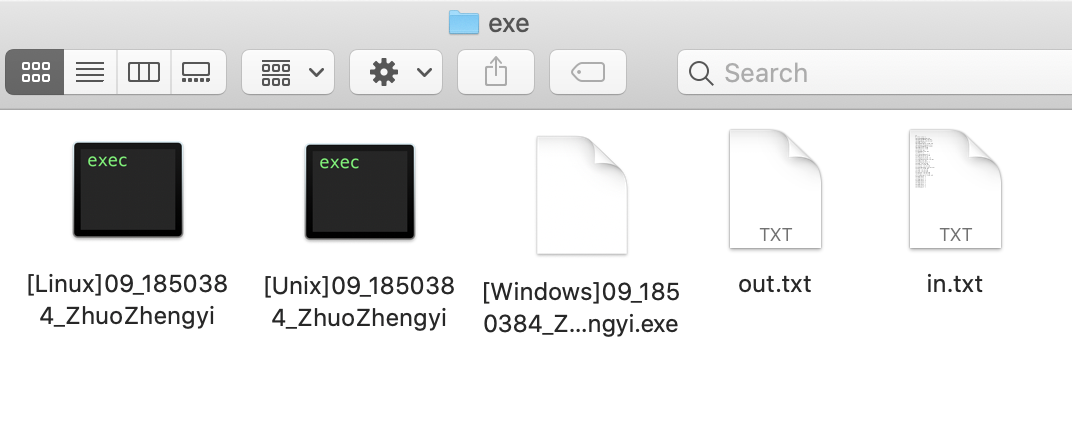
\includegraphics[width=11cm]{src/output.png}
    \caption{输出文件示意}
\end{figure}

\begin{figure}[H]
    \centering
    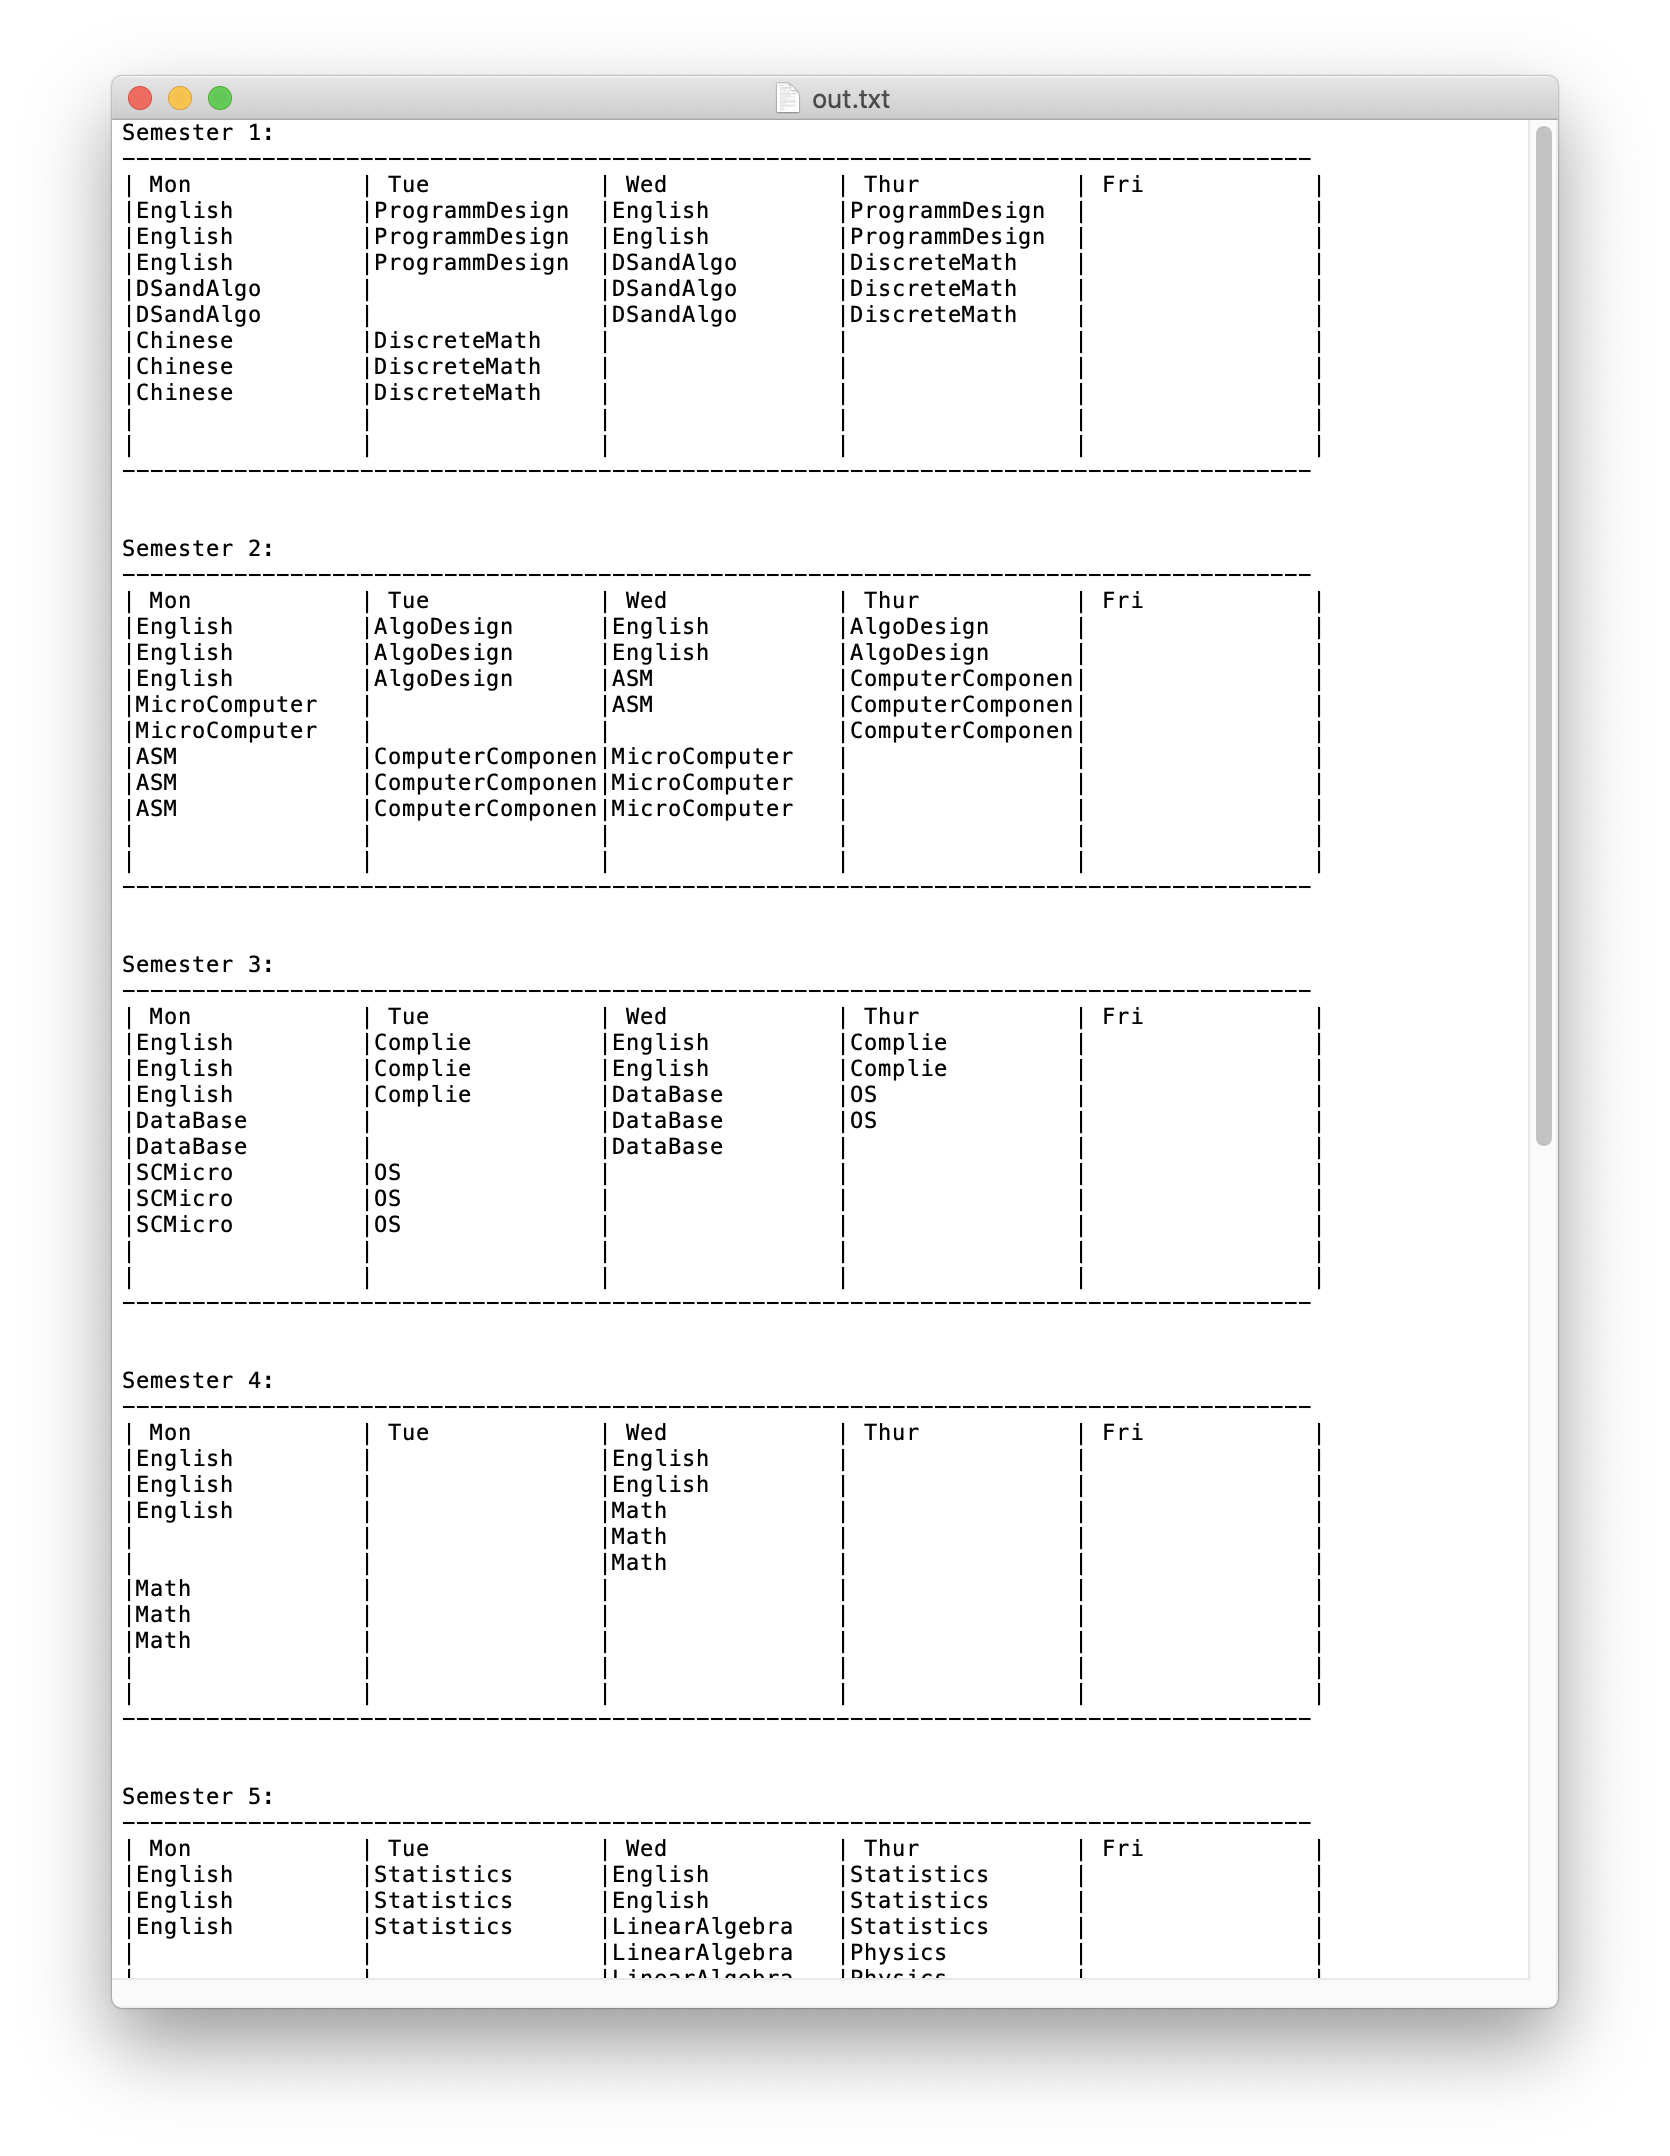
\includegraphics[width=11cm]{src/outputContent.png}
    \caption{输出文件内容}
\end{figure}


\backmatter
\lstlistoflistings
\listoffigures
\printindex
\end{document}